%%%%%%%%%%%%%%%%%%%%%%%%%%%%%%%%%%%%%%%%%
% Journal Article
% LaTeX Template
% Version 1.4 (15/5/16)
%
% This template has been downloaded from:
% http://www.LaTeXTemplates.com
%
% Original author:
% Frits Wenneker (http://www.howtotex.com) with extensive modifications by
% Vel (vel@LaTeXTemplates.com)
%
% License:
% CC BY-NC-SA 3.0 (http://creativecommons.org/licenses/by-nc-sa/3.0/)
%
%%%%%%%%%%%%%%%%%%%%%%%%%%%%%%%%%%%%%%%%%

%----------------------------------------------------------------------------------------
%	PACKAGES AND OTHER DOCUMENT CONFIGURATIONS
%----------------------------------------------------------------------------------------

\documentclass[14pt, a4paper]{article}
\usepackage[english, russian]{babel}
\usepackage{fontspec}
% \setmainfont{Times New Roman}

\setromanfont{Times New Roman}
\setsansfont{Arial}

% \usepackage{cyrtimes}

\usepackage{extsizes}
% \usepackage[T2A]{fontenc}
%
% \usepackage[utf8]{inputenc}

\usepackage{indentfirst}

%\usepackage{times}
\linespread{1.5}
\usepackage[left=30mm,right=15mm,top=15mm,bottom=20mm]{geometry}
\usepackage[framed,numbered,autolinebreaks,useliterate]{mcode}

\usepackage{graphicx, amsmath}
\numberwithin{figure}{section}
\graphicspath{{images/}}
\usepackage{amsfonts,amssymb}
\usepackage{caption}
\captionsetup[figure]{name=Рисунок, labelsep=endash}
\captionsetup[table]{labelsep=quad}

\numberwithin{equation}{section}

\usepackage{booktabs} % Horizontal rules in tables

\usepackage{lettrine} % The lettrine is the first enlarged letter at the beginning of the text

\usepackage{enumitem} % Customized lists
\setlist[itemize]{noitemsep} % Make itemize lists more compact

\usepackage{listings}
\usepackage{courier}
\usepackage{tocloft}
\usepackage{array}
\newcolumntype{H}{>{\setbox0=\hbox\bgroup}c<{\egroup}@{}}

\lstloadlanguages{Python}%,Clean,make,Fortran}%Загружаемые языки
\lstset{
	language=Python,                % choose the language of the code
	numbers=left,                   % where to put the line-numbers
	stepnumber=1,                   % the step between two line-numbers.
	numbersep=5pt,                  % how far the line-numbers are from the code
	backgroundcolor=\color{white},  % choose the background color. You must add \usepackage{color}
	showspaces=false,               % show spaces adding particular underscores
	showstringspaces=false,         % underline spaces within strings
	showtabs=false,                 % show tabs within strings adding particular underscores
	tabsize=2,                      % sets default tabsize to 2 spaces
	captionpos=b,                   % sets the caption-position to bottom
	breaklines=false,                % sets automatic line breaking
	breakatwhitespace=false,         % sets if automatic breaks should only happen at whitespace
	frame=none,
	basicstyle=\footnotesize\ttfamily
	%title=\lstname,                 % show the filename of files included with \lstinputlisting;
}

\usepackage{abstract} % Allows abstract customization
\usepackage{braket} % \bra{f}\ket
\usepackage{rotating}
\renewcommand{\abstractnamefont}{\normalfont\bfseries} % Set the "Abstract" text to bold
\renewcommand{\abstracttextfont}{\normalfont\small\itshape} % Set the abstract itself to small italic text
\newcommand{\sectionbreak}{\clearpage}
\newcommand*{\No}{\textnumero}
\renewcommand{\Re}{\mathrm{Re}}
\renewcommand{\Im}{\mathrm{Im}}

\newcommand{\const}{\mathrm{const}}
\newcommand{\arccosh}{\mathrm{arccosh}}

\newcommand{\vF}{\mathbf{F}}
\newcommand{\ve}{\mathbf{e}}
\newcommand{\vk}{\mathbf{k}}
\newcommand{\vq}{\mathbf{q}}
\newcommand{\vp}{\mathbf{p}}
\newcommand{\va}{\mathbf{a}}
\newcommand{\vP}{\mathbf{P}}
\newcommand{\vK}{\mathbf{K}}
\newcommand{\vQ}{\mathbf{Q}}
\newcommand{\vA}{\mathbf{A}}
\newcommand{\vr}{\mathbf{r}}
\newcommand{\vR}{\mathbf{R}}

\newcommand{\vRR}{\boldsymbol{\mathcal{R}}}
\newcommand{\veps}{\boldsymbol{\varepsilon}}

\newcommand{\cA}{\mathcal{A}}
\newcommand{\cR}{\mathcal{R}}
\newcommand{\cM}{\mathcal{M}}
\newcommand{\cE}{\mathcal{E}}
\newcommand{\cJ}{\mathcal{J}}
\newcommand{\cT}{\mathcal{T}}
\newcommand{\cD}{\mathcal{D}}
\usepackage{titlesec} % Allows customization of titles
% \renewcommand\thesection{\Roman{section}} % Roman numerals for the sections
% \renewcommand\thesubsection{\roman{subsection}} % roman numerals for subsections
\titleformat{\section}[block]{\normalsize\bfseries}{\thesection}{1ex}{}
\titleformat{\subsection}[block]{\normalsize\bfseries}{\thesubsection}{1ex}{}

\renewcommand{\cftsecleader}{\cftdotfill{\cftdotsep}}
\cftsetindents{section}{0em}{2em}
\cftsetindents{subsection}{0em}{2em}

\renewcommand\cfttoctitlefont{\hfill\normalsize\bfseries}
\renewcommand\cftaftertoctitle{\hfill\mbox{}}
\renewcommand\labelitemi{---}

\usepackage{hyperref} % For hyperlinks in the PDF

\addto\captionsrussian{\def\refname{Список использованных источников}}
\usepackage{setspace}
\onehalfspacing

\makeatletter
\renewcommand*{\@biblabel}[1]{#1}
\makeatother


\usepackage{titlesec}
\titleformat{\section}[block]{\normalsize\bfseries\centering}{\thesection}{1ex}{}
\titleformat{\subsection}[block]{\normalsize\bfseries}{\thesubsection}{1ex}{}
\titleformat{\subsubsection}[block]{\normalsize\bfseries}{\thesubsubsection}{1ex}{}
\usepackage[tocflat]{tocstyle}
%----------------------------------------------------------------------------------------
%	TITLE SECTION
%----------------------------------------------------------------------------------------


%----------------------------------------------------------------------------------------

\begin{document}
\tableofcontents
\section*{\centering Введение}
\addcontentsline{toc}{section}{Введение}
В данной работе рассматривается синтез ядер в астрофизических процессах. Процессы, приводящие к появлению легких элементов (с массовым числом меньше массового числа $Fe$) относительно известны и изучены. Однако распространенности элементов, тяжелее железа, относительно слабо зависит от массового числа A, что свидетельствует о ином механизме образования этих элементов. Образование такие ядер в результате взаимодействия заряженных частиц сильно подавлено из-за кулоновского барьера. Также большинство тяжелых элементов являются $\beta$-радиоактивными. На данный момент считается, что тяжелые элементы образуются в реакциях захвата нейтронов. Обычно различают быстрый (r) и медленный (s) процессы захвата нейтронов (от английских слов rapid и slow). Эти два механизма различаются отношением скорости захвата нейтронов (реакция (n, $\gamma$)) к скорости бета-распада. Предполагается, что примерно половина наблюдаемого количества элементов с A > 60 образуется в результате s-процесса. В настоящее время общепризнанно, что многие ядра тяжелее железа, включая все ядра тяжелее $^{209}Bi$, образуются r-процессом путем быстрого последовательного захвата большого количества нейтронов. Как было сказано выше, основное условие - высокая скорость захвата нейтронов. Однако эти условия (для возникновения r-процесса) являются экстремальными и встречаются крайне редко.  Считается, что такие условия наблюдаются в процесс слияния нейтронная звезда - нейтронная звезда.

Образование некоторых изотопов не может быть объяснено в рамках указанных выше процессов, их принято называть обойденными или p-изо\-то\-па\-ми. Их название обусловлено тем, что, если рассмотреть картину s-процесса и r-процесса, то можно увидеть стабильные элементы, которые не могут быть получены путем $\beta$-распада, так как в данных условиях, он не является разрешенным.

В данной работе моделируются реакции образования химических элементов в процессе поглощения нейтронной звезды черной дырой \cite{bhns1} с учетом столкновительного β-распада как процесса, приводящего к появлению обойденных ядер. Вычисление сечений реакций производится с использованием данных открытой библиотеки REACLIB, в основе которой лежит аппроксимация температурной зависмости сечения специальной фукнкцией, включающей 7 уникальных для каждой реакции параметров \cite{jina}.

Столкновительный бета-распад был впервые предложен в работе \cite{batkin}, объяснение образования обойденных элементов на
основе СБР - в работе \cite{tak}

В настоящей магистерской диссертации вычислены сечения СБР для ряда изотопов, а также найдены параметры температурной аппроксимации в формате библиотеки REACLIB. Полученные результаты включены в набор реакций, возникающих при поглощении нейтронной звезды черной дырой, и в дальнейшем выполнено моделирование синтеза химических элементов с помощью открытой библиотеки SkyNet \cite{skynet}. 

Процесс моделирования слияний нейтронная звезда - черная дыра будет выполняться с помощью открытой библиотеки SkyNet, написанную Jonas Lippuner с дополнение ее своим набором реакций.


\section{Проблема происхождения обойденных элементов}

Процессы, приводящие к происхождению элементов можно разделить на несколько видов. Большой взрыв привел к появлению водород ($\sim75\%$ общей массы) и гелий ($\sim25\%$) в промежутке от первых десяти секунд до минуты после большого взрыва, а также некоторое количество дейтерия, $^3H$e и $^7Li$ \cite{Tytler}.

 Далее происходило горении в звездах малой массы, представляющее из себя p-p-цепь, имеющую малое сечение, приводящее к появлению более тяжелых элементов, таких как $^{20}Ne$, $^{24}Mg$, $^{28}Si$ и т. д. \cite{cauldrons, energy, interiors}. 
 
 Звезды с начальной массой более $8 M_\odot$ проходят через несколько стадий горения, которые в конечном счете могут произвести элементы вплоть до массового числа А = 56 (когда энергия связи на нуклон (протоны и нейтроны) достигает максимума). Поэтому более тяжелые нуклиды связаны слабее, что означает, нужно добавить энергию, для обеспечения слияние за пределами A = 56 \cite{cauldrons, qse, massive}. Из-за кулоновского барьера распространенность элементов до пика железа намного выше распространенности более тяжелых нуклидов \cite{iron-abu}.
 
 Процесс приводящий к появлению элементов за пиком железа - захват нейтронов \cite{cauldrons}. В зависимости от того, является ли время $\tau_\beta$ для $\beta$-распада короче или длиннее чем время $\tau_n$ для захвата нейтронов, выделяют r-процесс и s-процесс.
 
 R-процесс приводит к появлению элементов с большим массовым числом, однако требует экстремальных условий и места его протекания до сих пор исследуются. Поскольку сечение захвата нейтронов должно быть велико, требуется очень богатая нейтронами среда \cite{places}. Недавние исследования показывают, что коллапс ядра сверхновых и слияние нейтронных, слияние черной дыры - нейтронной звезд являются единственными жизнеспособными кандидатами на места протекания r-процесса \cite{sites, neutrino, nsns, bhns1}. 
 
 Совсем недавно, было обнаружен коллапсара, который также является местом протекания r-процесса \cite{collapsars}.
 
Однако ни r-процесс, ни s-процесс не объясняют происхождение некоторых ядер, так как $\beta$-распад, необходимый для их появления, является запрещенным, если смотреть на траекторию преобразования элементов. Такие ядра называют обойденными или p-ядрами. Их происхождение до сих пор малоизучено \cite{p-process}.

Обойдённые ядра - устойчивые атомные ядра, лежащие в стороне от всех возможных путей образования тяжёлых ядер из более лёгких в процессе последовательного захвата последними нейтронов \cite{reactions}. Распространённость обойденных ядер, как правило, примерно на два порядка величины ниже, чем у близких к ним ядер, лежащих на пути нейтронного захвата. К таковым относятся: $^{74}Se$, $^{78}Kr$, $^{80}Kr$, $^{84}Sr$, $^{92}Mo$, $^{94}Мо$, $^{96}Ru$, $^{98}Ru$, $^{102}Pd$, $^{106}Cd$, $^{108}Cd$, $^{113}In$, $^{112}Sn$, $^{114}Sn$, $^{115}Sn$, $^{120}Te$, $^{124}Xe$, $^{126}Xe$, $^{130}Ba$, $^{132}Ba$, $^{136}Ce$, $^{138}Ce$, $^{144}Sm$, $^{152}Gd$, $^{152}Dy$, $^{158}Dy$, $^{162}Er$, $^{164}Er$, $^{168}Yb$, $^{174}Hf$, $^{180}W$, $^{184}Os$, $^{190}Pt$, $^{196}Hg$ \cite{role}.

\section{SkyNet}

Программный пакет SkyNet представляет из себя универсальную сеть ядерных реакций, специально разработанную для моделирования r-процесса, но она также применима к другим астрофизическим сценариям \cite{skynet}.

В качестве библиотеки ядерных реакций в данном программном обеспечении используются данные формата открытой базы реакций JINA REACLIB.  Данная баз хранит показатели реакций, таких как зависимость от температуры через семи-параметрическое приближение \cite{jina}, тип реакции (резонирующая, нерезонирующая, слабая, спонтанный распад), значение температуры, переданное среде, а также параметр $v$, указывающий, являются ли показатели $a_0, .., a_6$ обратными. В подавляющем большинстве реакций показатели представляют из себя параметризацию сечения в зависимости от температуры:

\begin{equation}
\label{eq:system}
\begin{split}
\left.
\begin{array}{ccc}
N_{A}\langle \sigma v \rangle \\
\lambda_\gamma
\end{array}
\right\}
= \exp (a_0 + a_1 T_9^{-1} + a_2 T_9^{-1/3} + \\
a_3 T_9^{1/3} + a_4 T_9 + a_5 T_9^{5/3} + a_6 \ln T_9)
\end{split}
\end{equation}

SkyNet позволяет расширять список реакций, используемый при моделировании астрофизических явлений путем добавления новых файлов в сеть. Таким образом, меняя параметры моделирования можно оценить влияния тех или иных реакций на распространенности элементов.


\section{Столкновительный β-распад}
Данный процесс является одним из процессов, приводящих к появлению обойденных ядер. Впервые данный процесс был предложен в работе \cite{batkin}. 

Столкновительный $\beta-$распад стабильных ядер, инициируемый их кулоновскими столкновениями с другими ядерными частицами звездной среды, может быть основой модели процесса синтеза обойденных ядер.
Проблема их синтеза на основе физического механизма захвата нейтронов ($s-$ или $r-$процесса) состоит в прерывании цепочки последовательных $\beta-$распадов на $\beta$-стабильном ядре $(A,Z)$.

Процесс СБР стабильных ядер, о котором говорилось выше, для нуклидов главной последовательности предоставляет еще одну возможность преодолеть энергетический порог и осуществить переход 
$$(A,Z) \xrightarrow[]{\beta^-} (A,Z + 1),$$
открывая путь к последующему естественному $\beta$-переходу
$$(A,Z+1) \xrightarrow[]{\beta^-} (A,Z + 2)$$

Расчеты показывают, что модель синтеза обойденных элементов в звездном веществе на этапе квазиравновесной стадии, основанная на явлении СБР стабильных ядер главной последовательности, качественно, а в ряде случаев и количественно, способна воспроизвести нерегулярный ход кривой относительной распространенности обойденных ядер. Этот факт можно расценивать как косвенное свидетельство в пользу реальности явления столкновительного $\beta$-распада стабильных ядер \cite{tak}.

В случае столкновительного $\beta$-распада возможно несколько видов процессов, а именно: протон-ядерные, ядро-ядерные и процесс, стимулированный нейтронами. Рассчитанные сечения для протон-ядерных и ядро-ядерных оказались невелики (менее $10^{-50}cm^2$), и процесс пока не доступен для прямого наблюдения, но при помощи программного обеспечения, позволяющего моделировать данные процессы мы можем оценить влияние их на конечные распространенности элементов \cite{tak_article}. Наряду с кулоновскими столкновениями ядер можно предложить механизм СБР, не связанный с кулоновскими силами и в то же время незамаскированный возможным появлением продуктов $\beta$-распада за счет ядерных реакций. Речь идет о процессе СБР ядра, стимулированном столкновениями с нейтронами.

Сечение для столкновительного $\beta$-распада при столкновении частицы с протоном или другой частицей имеет вид:

\begin{multline} \label{sech}
\sigma^{(col)}_\beta(\beta_f)=
{4\sqrt{2}\over \pi} {{g^2_v\alpha_e^4Z (Z+1) {Z'}^4 \mu^{9/2}}
	\over{\varepsilon_i^{3/2} (1-exp(-2\pi\lambda_i))}}
\xi_\beta(\beta_f)
\times\\
\times\int\limits_0^{\varepsilon_i{-}\Delta{-}\Delta_f}\!\!\!\!\!
{{\Phi(E_f) d\varepsilon_f}\over{(exp(2\pi\lambda_f)-1)
		k_f ( k_i- k_f)^4(k_i+k_f)^2}}\times\\
\times\int\limits_{x_0}^0 {{|{\rm F}(-i \lambda_i, -i\lambda_f,1; x)|^2}\over{(1-x)^2}} dx,
\end{multline}

\subsection{Постановка задачи r-процесса}

Целью данной работы является оценка вклада столкновительного $\beta$-распада на происхождение обойденных элементов. Для этого смоделируем при помощи SkyNet слияние черной дыры и нейтронной звезды (BHNS) с использование заранее известных параметров системы \cite{bhns}.

Начальный состав представляет из себя $T = 6.1 \text{ГК}$, $\rho = 7.4 \times 10^9 \text{г} \text{см}^{-3}$, и $Y_e = 0.07$. Большую часть элементов составляют нейтроны ($\sim 79 \%$), поэтому дальнейшие исследования зависимости происхождения p-элементов от столкновения с нейтронами, должны дать более значительный результат. Для столкновения с протоном мы выбрали именно эту систему для моделирования, так как эволюция данного процесса протекает на большом отрезке времени, что дает большее расхождения на конечном этапе эволюции. Временной отрезок здесь от $10^{-3}\text{с}$ до $5\times10^8\text{с}$.

Для непосредственной оценки влияний СБР построим сечения реакций, приводящий к появлению обойденных элементов, параметризуем их для приведения к формату JINA REACLIB и добавим в сеть.

В конечном итоге сравним распространенности обойденных элементов с учетом СБР и без его учета.

\section{Аппроксимация}

Сначала построим сечения для солкновения некоторых элементов с протоном. Для этого воспользуемся параметрами из таблицы \ref{Tels}. 

\begin{table}
	\centering
	\caption{Характеристики праматеринских ядер.}
	\tabcolsep=5pt
	\begin{tabular}{|c|c|c|HHc|c|}
		\hline
		Праматеринское& Материнское & Обойденное &$\; J_i\; $&$J_f$&$\Delta + \Delta_f,$&${\rm lg} f_0t$\\
		ядро  &   ядро & ядро &&&$\text{МэВ}$&\\
		\hline
		$^{74}Ge$ & $^{74}As$ &$^{74}Se$ & $0^+$  &  $(1^+)$ & 2,766 &      \\
		$^{74}Ge$ & $^{74}As$ &$^{74}Se$& $0^+$  &  $(1^+)$ & 2,982 &      \\
		$^{78}Se$ & $^{78}Br$ &$^{78}Kr$& $0^+$  &  $1^+$  & 3,5737 &   4,8   \\
		$^{80}Se$ & $^{80}Br$ &$^{80}Kr$& $0^+$  &  $1^+$  & 1,8703 &   4,6  \\
		$^{84}Kr$ & $^{84}Rb$ &$^{84}Sr$& $0^+$  &  $2^-$  & 2,68   &   9,6  \\
		$^{106}Pd$ & $^{106}Ag$ &$^{106}Cd$& $0^+$  &  $1^+$  & 2,983 &   4,9   \\
		$^{106}Pd$ & $^{106}Ag$ &$^{106}Cd$& $2^+$  &  $1^+$  & 2,471 &   5,3   \\
		$^{108}Pd$ & $^{108}Ag$ &$^{108}Cd$& $0^+$  &  $1^+$  & 1,921 &   4,8   \\
		$^{108}Pd$ & $^{108}Ag$ &$^{108}Cd$& $2^+$  &  $1^+$  & 1,487 &   5,5   \\
		$^{112}Cd$ & $^{112}In$ &$^{112}Sn$& $0^+$  &  $1^+$  & 2,578 &   4,7   \\
		$^{112}Cd$ & $^{112}In$ &$^{112}Sn$& $2^+$  &  $1^+$  & 1,961 &   5,3   \\
		$^{114}Cd$ & $^{114}In$ &$^{114}Sn$& $0^+$  &  $1^+$  & 1,9846 &   4,8   \\
		$^{114}Cd$ & $^{114}In$&$^{114}Sn$ & $2^+$  &  $1^+$  & 1,4266 &   5,3   \\
		$^{120}Sn$ & $^{120}Sb$ &$^{120}Te$& $0^+$  &  $1^+$  & 2,681 &   4,5   \\
		$^{124}Te$ & $^{124}I$  &$^{124}Xe$& $0^+$  &  $2^-$  & 3,157 &   9,3   \\
		$^{124}Te$ & $^{124}I$  &$^{124}Xe$& $2^+$  &  $2^-$  & 2,555 &   7,5   \\
		$^{126}Te$ & $^{126}I$  &$^{126}Xe$& $0^+$  &  $2^-$  & 2,156 &   9,2   \\
		$^{126}Te$ & $^{126}I$ &$^{126}Xe$ & $2^+$  &  $2^-$  & 1,49 &   7,4   \\
		$^{130}Xe$ & $^{130}Cs$ &$^{130}Ba$& $0^+$  &  $1^+$  & 3,019 &   5,1   \\
		$^{130}Xe$ & $^{130}Cs$ &$^{130}Ba$& $2^+$  &  $1^+$  & 2,483 &   6,4   \\
		$^{132}Xe$ & $^{132}Cs$ &$^{132}Ba$& $2^+$  &  $2^{(-)}$  & 1,443 &   6,0   \\
		$^{136}Ba$ & $^{136}La$ &$^{136}Hf$& $0^+$  &  $1^+$  & 2,87 &   4,6   \\
		$^{164}Dy$ & $^{164}Ho$ &$^{164}Er$& $0^+$  &  $1^+$  & 1,0292 &   4,6   \\
		$^{164}Dy$ & $^{164}Ho$ &$^{164}Er$& $2^+$  &  $1^+$  & 0,9558 &   4,9   \\
		\hline
	\end{tabular}
	\label{Tels}
\end{table}

Сечение каждой реакции были посчитаны для набора из 24 температур: $T_9$ = 0.1,0.15, 0.2, 0.3, 0.4, 0.5, 0.6, 0.7, 0.8, 0.9, 1.0, 1.5, 2.0, 2.5, 3.0, 3.5, 4.0, 4.5, 5.0, 6.0, 7.0, 8.0, 9.0, 10.0 ($T = T_9 \times 10^{9}\text{К}$). Так как данный набор является избыточным для параметризации вида \ref{eq:system}, воспользуемся методом наименьших квадратов. 

\begin{figure}[ht]
	\center{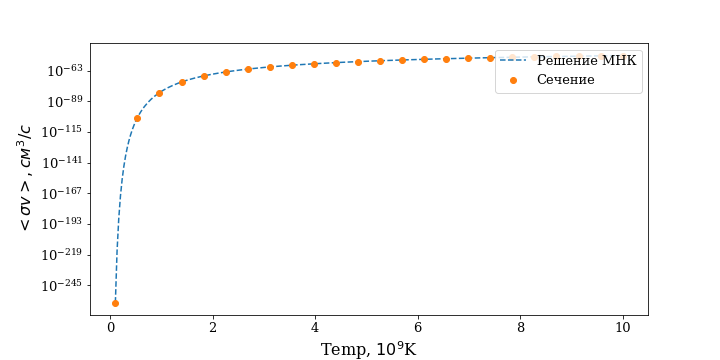
\includegraphics[width=0.8\linewidth]{compare-xe130-cs130}}
	\caption{Сравнение решения методом наименьших квадратов с расчитанным сечением}
	\label{ris:2}
\end{figure}

Далее, составим необходимый для REACLIB файл библиотеки реакций. Для перехода $^{130}Xe \to ^{130}Cs$ получаем строки вида: 

\begin{lstlisting}[label={lst:label}]
5
pxe130cs130    p                  cleaw     0.00000e+00          
3.631089e+01-2.513083e+01-3.379005e+02 1.434772e+02                      
-2.028014e+00-6.306473e-02-1.208779e+02                                   

\end{lstlisting}


\section{Анализ результатов}

\begin{sidewaysfigure}[ht]
	\center{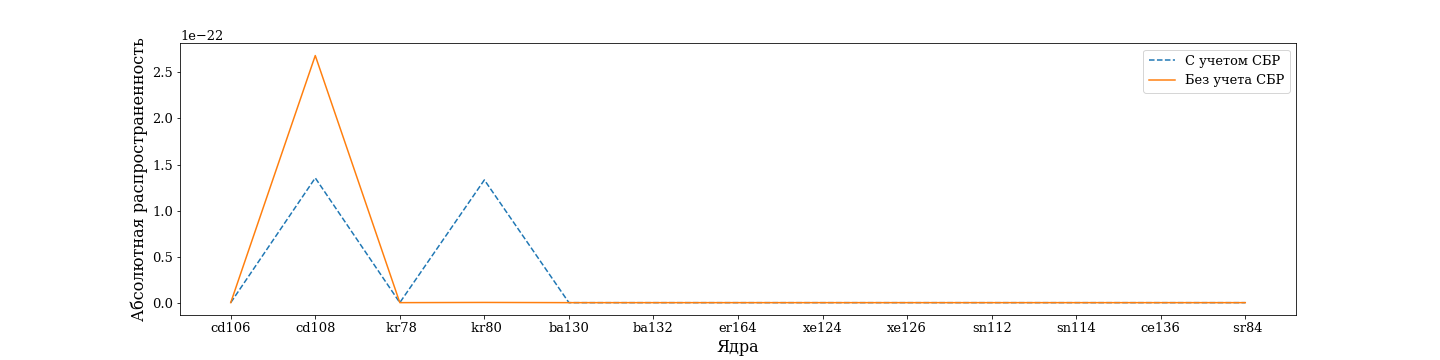
\includegraphics[width=1\linewidth]{result}}
	\caption{Конечные распространенности обойденных ядер с исходной библиотекой (синий график), и библиотекой, включающей СБР (розовой график)}
	\label{ris:result}
\end{sidewaysfigure}

Самое важным на данном графики является то, что, несмотря на ожидание увидеть меньшие распространенности всех элементов, мы наблюдаем то, что для некоторых ядер это разница несущественна $^{114}Sn$. Более того, наблюдается относительный избыток ядер $^{78}Kr$ и $^{80}Kr$.

Построим график относительной ошибки между эволюцией элементов с нашей библиотекой реакций и тем, что присутствовало в изначальной версии REACLIB (рисунок \ref{ris:result-err}):

\begin{sidewaysfigure}[ht]
	\center{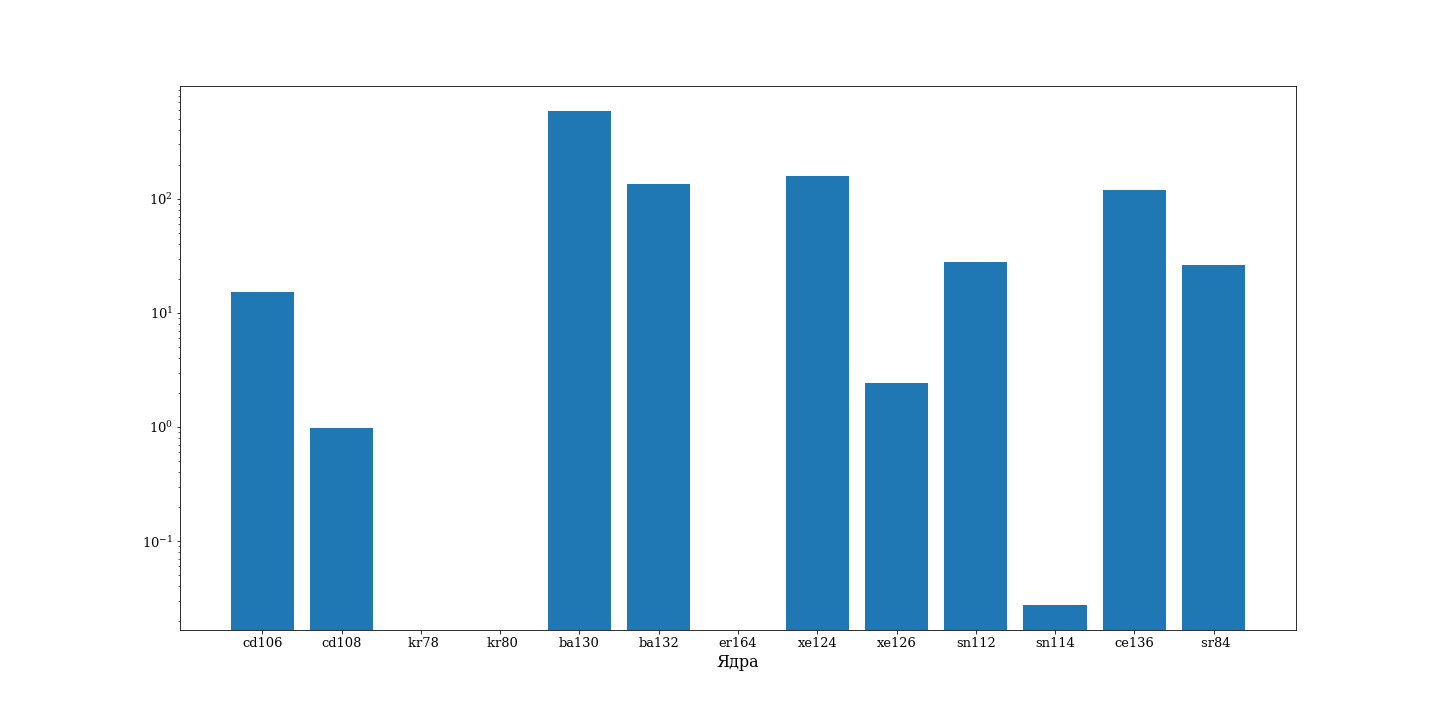
\includegraphics[width=1\linewidth]{result-err}}
	\caption{Относительная разница при сравнении результатов моделирования со стандартной библиотекой реакций SkyNet и библиотекой, учитывающей только СБР для образования обойденных изотопов}
	\label{ris:result-err}
\end{sidewaysfigure}

\section*{\centering Заключение}
\addcontentsline{toc}{section}{Заключение}
В данной работе было рассмотрено влияние столкновительного бета-распада на синтез химических элементов.

Сначала мы вычислили сечения столкновительного бета рас-пада для реакций из таблицы \ref{Tels}, а именно, столкновения протона с праматеринским ядром. Для этого была написана программа на языке Python, позволяющая получить сечение, имея небольшое количество начальных данных.

Данные сечения были параметризированны через 7 параметров $a_0, ..., a_6$, определяющих зависимость от температуры, чтобы иметь возможность дополнить реакциями библиотеку JINA REACLIB. Из полученных наборов параметров, был построен файл, который представляет из себя реакции REACLIB для каждого из процессов таблицы \ref{Tels}.


Далее, при помощи пакета SkyNet были приведено моделирование слияние черной дыры-нейтронной звезды, чтобы оценить влияние СБР на общую картину распространенностей элементов. Моделирование проводилось дважды, сначала - с немодифицированной библиотекой JINA REACLIB, затем - с модифицированной, в которую были включены реакции $$\text{праматеринское ядро} \to \text{материнское ядро}.$$

Было выплнено сравнение полученных картин распространенностей элементов.  Сравнение производилось только лишь для обойденных элементов, так как именно их происхождения является темой данной работы. Было подтверждено, что СБР может являться источником обойденных ядер и при больших концентрациях протонов (в условиях рассматриваемого процесса) это влияние суще-ственно, более того, мы можем также получить избыток некоторых элементов.

В данной работе рассматривается образование материнских ядер только при столкновениях с протономи. В дальнейшем предполагается учесть вклад СБР с другими ядрами и нейтронами (отсутствие кулоновско-го барьера), что должно увеличить суммарное сечение СБР, приводящее к появлению обойденных элементов, что даст иную результирующую картину.

\newpage
\addcontentsline{toc}{section}{Список используемой литературы}
\bibliographystyle{ugost2003}
\bibliography{sample}

\end{document} 